\subsection{Setup}
Dasgupta et al. \cite{dasgupta2012social} performed various experiments to compare the performance of the presented samplers.
They focused on two large, publicly available databases \texttt{LiveJournal} and \texttt{DBLP}.

The \texttt{LiveJournal} network contains 5.36M nodes and approximately 160M edges and is based on a snapshot of the social network \url{http://livejournal.com} in March 2008. In addition to the network they extracted the users age, location (city, state, country) and a list of interests where available on the users public profile.
The \texttt{DBLP} network contains 368K nodes and 8M edges and consists of the content of the DBLP database located at \url{http://www.informatik.uni-trier.de/~ley/db/}. The nodes stand for authors while the edges represent co-authorship on some publication. The node attributes are formed by the authors publication venues, however only the a random set of 100 venues with probability proportional to their popularity were considered. 

Since the samplers have been designed keeping the Definition \ref{defsampler} in mind, recall that they provide an additive $\epsilon$-approximation. So most importantly we measure the absolute error of each sampler with respect to the true value. If our estimator outputs $\hat{f}$ approximating $\bar{f}$ we measure the error as $|\bar{f}-\hat{f}|$.

To get a relation between error and sample size we vary the sample size $r$ from a minimum of $r = 100$ to $r = 50000$. We use the distributions mentioned in chapter \ref{algorithms}: uniform at random (\texttt{unif}), proportional to the degree of the node (\texttt{deg}) and additionally, proportional to the square root of the degree of the node (\texttt{sqrtdeg}). 
We omit any other combinations of algorithm and distributions since they almost always did not result in better performance and are computationally more expensive. 
\subsection{Performance on LiveJournal}
For analyzing the performance on LiveJournal we are interested in a set of five cities, five states, five countries, a set of ages, age-buckets and a set if interests (sports) each with a typical size ranging from 0.4\% to 4\%.
The correlation between number of samples and absolute error for the presented samplers is displayed in \rfig{livejournal1}. 
%---figure network a------------------------------------
\begin{figure}[!ht]
  \begin{center}
    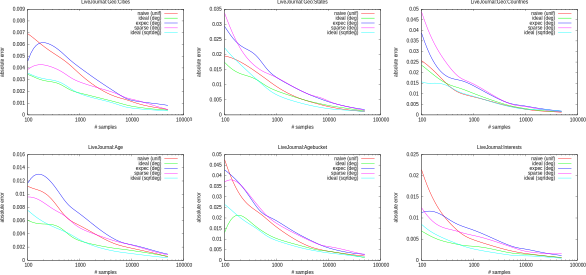
\includegraphics[width=\linewidth]{fig2_3}
    \caption{\#samples vs error of various samplers on the LiveJournal data}
    \lfig{livejournal1} 
  \end{center}
\end{figure}
%---end figure network a--------------------------------
\subsection{Performance on DBLP}
In DBLP we were interested in 100 venues of publication ranging in size from 0.01\% to 3\% in size.

The improvements offered by \texttt{Ideal} over \texttt{Naive} are even larger. In comparison the \texttt{Naive} sampler requires at least 3-5 times more samples than \textit{Ideal} for achieving the same error.
%---figure network a------------------------------------
\begin{figure}[!ht]
  \begin{center}
    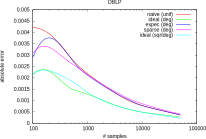
\includegraphics[width=0.5\linewidth]{fig4}
    \lfig{dblp}
  \end{center}
\end{figure}
%---end figure network a--------------------------------
\subsection{Effect of sparsity parameter}
When designing the \texttt{Sparse} sampler Alg. \ref{algsparse} we introduced a new parameter $k$ which we call the sparsity parameter since it defines the amount of the picked neighbors.
The measurements show that using $k=9$ seems to be almost as good as sampling only three neighbors.
%---figure network a------------------------------------
\begin{figure}[!ht]
  \begin{center}
    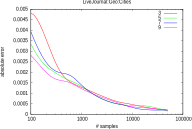
\includegraphics[width=0.5\linewidth]{fig7b}
    \lfig{sparsity}
  \end{center}
\end{figure}
%---end figure network a--------------------------------
